% !TEX root = ../vr_st.tex

\subsection{Real projective spaces}\label{s:critical_radii_rpn}

Let us now focus on the real equatorial system with the antipodal action.
We will consider every sphere \(\bS^n(2)\) to have radius 2 so the quotient \(\rp^n\) has the same diameter as \(\bS^n\).
We will consider reduced (co)homology with mod 2 coefficients.

\medskip\lemma
For \(k,n,m \in \N\) and \(\Sq^k \in \cO(m-k, m)\) we have:
\begin{enumerate}
	\item \(\crit(\rp^n) = \frac{\pi}{3}\).
	\item \(\firstdeath{m}{\rp^n} =
	\begin{cases}
		\frac{\pi}{3} & m \leq n, \\
		\hfil 0 & \text{otherwise}.
	\end{cases}\)
	\item \(\firstdeath{\Sq^k}{\rp^n} =
	\begin{cases}
		\tfrac{\pi}{3} & k \leq \frac{n-1}{2} \text{ and } \binom{m-k}{k} \text{ is odd},\\
		\hfil 0 & \text{otherwise}. \\
	\end{cases}\)
\end{enumerate}

\begin{proof}
	(1) This part is stated and proven in \cite[Thm.~4.5]{adams2022metric}.

	(2) We only need to prove for the case of $m\leq n$, since the other case follows from the definition since \(\rH_m(\rp^n) = 0\) if \(m > n\) or \(m = 0\).

    Consider the \(\rC_2\)-action on the real equatorial system \(\bS^{1}(2) \to \bS^{2}(2) \to \dotsb \to \bS^{n}(2)\), where each $\bS^{i}(2)$ is the $i$-sphere with radius $2$.
    By \cref{subsub:system VR compatible}, this system is \(\VR\)-compatible.
    By \cite{katz1983filling}, the filling radius of $\rp^i = \bS^{i}(2)_{\rC_2}$ is $\frac{\pi}{3}$ for any $i \geq 1$, which implies that $\fillrad(\rp^i)$ is non-decreasing as a function of \(i\).
    Therefore, we can apply \cref{ss:fundamental_lemma} to deduce that for any \(m \leq n\),
    \[
    \firstdeath{m}{\rp^n} \leq \fillrad(\rp^n) = \tfrac{\pi}{3}.
    \]
	On the other hand, $\firstdeath{m}{\rp^n}\geq \crit(\rp^n) = \tfrac{\pi}{3}$.
    Thus, the equality holds.

	(3) We only need a proof for the case $k \leq \frac{n-1}{2}$ and $\binom{m-k}{k}$ odd, since \(\Sq^k = 0\) otherwise.
	Because $\crit(\rp^n)=\frac{2\pi}{3}$, $\VR_r(\rp^n)$ retains the homotopy type of $\rp^n$ for $r \in (0,\tfrac{2\pi}{3})$.
    Recall from \cref{sss:cohomology_rpn} the cohomology algebra \(\rH^\ast(\rp^n; \Ftwo) \cong \frac{\Ftwo[\sigma]}{(\sigma^{n+1} = 1)}.\)
    Thus, $\Sq^k(\sigma^{m-k}) = \sigma^{m}$ generates a bar in the $\img_{\Sq^k}$-barcode that is born at $0$ and stays alive until the non-trivial class $\sigma^{m}$ dies at $\tfrac{2\pi}{3}$.
	Thus, $\firstdeath{\Sq^k}{\rp^n} \leq \tfrac{\pi}{3}$.
	On the other hand, $\firstdeath{\Sq^k}{\rp^n} \geq \crit(\rp^n) = \tfrac{\pi}{3}$.
\end{proof}

Using the above values, the estimates resulting from the analysis of \cref{ss:barcode_general} are illustrated in \cref{fig:sq barcodes}.

\begin{figure}
	\centering
	\begin{tikzpicture}[scale=0.52]
	\begin{axis} [
		title = {\LARGE $\Hbarc{m}{\rp^n},\, m\leq n$},
		ticklabel style = {font=\Large},
		axis y line=middle,
		axis x line=middle,
		ytick={0.5,0.67,0.95},
		yticklabels={$\frac{\pi}{2}$,$\frac{2\pi}{3}$,$\pi$},
		xtick={0.5,0.67,0.95},
		xticklabels={$\frac{\pi}{2}$,$\frac{2\pi}{3}$,$\pi$},
		xmin=-0.015, xmax=1.1,
		ymin=0, ymax=1.1,]
		\addplot [mark=none] coordinates {(0,0) (1,1)};
		\addplot [thick,color=black!20!white,fill=black!30!white,
		fill opacity=0.4]coordinates {
			(0.67,0.95)
			(0.67,0.67)
			(0.95,0.95)
			(0.67,0.95)};
		\addplot [black!40!white,mark=none,dashed, thin] coordinates {(0,0.67) (0.67,0.67)};
		%\addplot [black!40!white,mark=none,dashed, thin] coordinates {(0,0.72) (0.72,0.72)};
		\addplot [black!40!white,mark=none,dashed, thin] coordinates {(0.67,0) (0.67,0.67)};
		\addplot[barccolor,mark=*] (0, 0.67) circle (2pt) node[above right,barccolor]{};%{\Large\textsf{1}};
		%\node[mark=none] at (axis cs:0.68,0.21){$\Hbarc{1}{\rp^n}$};
	\end{axis}
\end{tikzpicture}
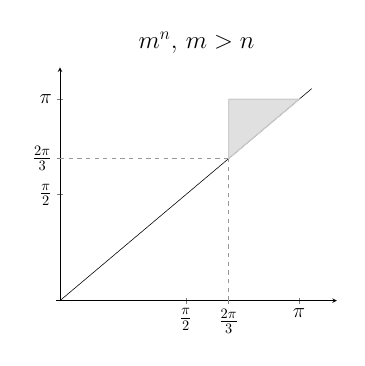
\begin{tikzpicture}[scale=0.52]
	\begin{axis} [
		title={\LARGE $\Hbarc{m}{\rp^n},\, m>n$},
		ticklabel style = {font=\Large},
		axis y line=middle,
		axis x line=middle,
		ytick={0.5,0.67,0.95},
		yticklabels={$\frac{\pi}{2}$,$\frac{2\pi}{3}$,$\pi$},
		xtick={0.5,0.67,0.95},
		xticklabels={$\frac{\pi}{2}$,$\frac{2\pi}{3}$,$\pi$},
		xmin=-0.015, xmax=1.1,
		ymin=0, ymax=1.1,]
		\addplot [mark=none] coordinates {(0,0) (1,1)};
		\addplot [thick,color=black!20!white,fill=black!30!white,
		fill opacity=0.4]coordinates {
			(0.67,0.95)
			(0.67,0.67)
			(0.95,0.95)
			(0.67,0.95)};
		\addplot [black!40!white,mark=none,dashed, thin] coordinates {(0,0.67) (0.67,0.67)};
		\addplot [black!40!white,mark=none,dashed, thin] coordinates {(0.67,0) (0.67,0.67)};
		% \addplot[barccolor,mark=*] (0, 0.67) circle (2pt) node[above right,barccolor]{\Large\textsf{1}};
		% \node[mark=none] at (axis cs:0.68,0.21){$\Hbarc{m}{\rp^n},\, m\geq 2$};
	\end{axis}
\end{tikzpicture}

\begin{tikzpicture}[scale=0.52]
	\begin{axis} [
		title = {\LARGE $\sqbarcl{k}{}{\rp^n},\, m \leq n$ and $\binom{m-k}{k}$ odd},
		ticklabel style = {font=\Large},
		axis y line=middle,
		axis x line=middle,
		ytick={0.5,0.67,0.95},
		yticklabels={$\frac{\pi}{2}$,$\frac{2\pi}{3}$,$\pi$},
		xtick={0.5,0.67,0.95},
		xticklabels={$\frac{\pi}{2}$,$\frac{2\pi}{3}$,$\pi$},
		xmin=-0.015, xmax=1.1,
		ymin=0, ymax=1.1,]
		\addplot [mark=none] coordinates {(0,0) (1,1)};
		\addplot [thick,color=black!20!white,fill=black!30!white,
		fill opacity=0.4]coordinates {
			(0.67,0.95)
			(0.67,0.67)
			(0.95,0.95)
			(0.67,0.95)};
		\addplot [black!40!white,mark=none,dashed, thin] coordinates {(0,0.67) (0.67,0.67)};
		%\addplot [black!40!white,mark=none,dashed, thin] coordinates {(0,0.72) (0.72,0.72)};
		\addplot [black!40!white,mark=none,dashed, thin] coordinates {(0.67,0) (0.67,0.67)};
		\addplot[barccolor,mark=*] (0, 0.67) circle (2pt) node[above right,barccolor]{};
        %{\Large$\geq$\textsf{1}};
	\end{axis}
\end{tikzpicture}
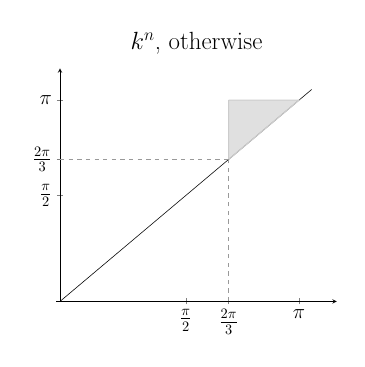
\begin{tikzpicture}[scale=0.52]
	\begin{axis} [
		title={\LARGE $\sqbarcl{k}{}{\rp^n}$, otherwise},
		ticklabel style = {font=\Large},
		axis y line=middle,
		axis x line=middle,
		ytick={0.5,0.67,0.95},
		yticklabels={$\frac{\pi}{2}$,$\frac{2\pi}{3}$,$\pi$},
		xtick={0.5,0.67,0.95},
		xticklabels={$\frac{\pi}{2}$,$\frac{2\pi}{3}$,$\pi$},
		xmin=-0.015, xmax=1.1,
		ymin=0, ymax=1.1,]
		\addplot [mark=none] coordinates {(0,0) (1,1)};
		\addplot [thick,color=black!20!white,fill=black!30!white,
		fill opacity=0.4]coordinates {
			(0.67,0.95)
			(0.67,0.67)
			(0.95,0.95)
			(0.67,0.95)};
		\addplot [black!40!white,mark=none,dashed, thin] coordinates {(0,0.67) (0.67,0.67)};
		\addplot [black!40!white,mark=none,dashed, thin] coordinates {(0.67,0) (0.67,0.67)};
	\end{axis}
\end{tikzpicture}
	\caption{Let $m \in \N$ and $\Sq^k \in \cO(m-k, k)$.
        \emph{Top row:} the persistent reduced homology barcode of $\rp^n$.
		%When $1\leq \degp \leq n$, the barcode consists of one $(0,\frac{2\pi}{3})$ and potentially some bars dominated by $(\frac{2\pi}{3}, \pi)$.
		\emph{Bottom row:} the $\img_{\Sq^k}$-barcode of $\rp^n$.
		%The leftmost barcode contains at least one $(0,\frac{2\pi}{3})$ and potentially some bars dominated by $(\frac{2\pi}{3}, \pi)$;
        %See \cref{s:critical_radii_rpn} for details.
        In each figure, the gray region represents where additional bars could exist within the corresponding barcode.
	}
	\label{fig:sq barcodes}
\end{figure}

\subsection{Lens spaces}\label{s:critical_radii_lens}

Much less information is known about Lens spaces.
We are interested in spheres \(\bS^{2n+1}(p)\) of radius \(p\), so the quotient \(\rL_p^n\) has the same diameter as \(\bS^{2n+1}\).
We will consider reduced (co)homology with mod \(p\) coefficients.

\medskip\lemma 
For fixed $n\in \N$, if $\fillrad(\rL^1_p) \leq \dotsb \leq \fillrad(\rL^n_p) < \tfrac{3\zeta_{2n+1}}{4}$, then for any non-negative degree $m\leq 2n+1$, 
\[
\firstdeath{m}{\rL^n_p} \leq \tfrac{\zeta_{2n+1}}{4} + \tfrac{\zeta_{m}}{2}.
\]

\begin{proof}
    It is enough to consider odd homology degrees, since $\firstdeath{m}{\rL^n_p} = 0$ when $m$ is even.
    For odd degrees, we apply an argument similar to that in the second part of the proof of \cref{s:critical_radii_rpn}.
    By \cref{subsub:system VR compatible}, the $\rC_p$-action on the system $\bS^1(p) \subset \bS^3(p) \subset \dotsb \subset \bS^n (p)$ is \(\VR\)-compatible. \ling{verify the consistence of radius}
    This, combined with the assumption that $\fillrad(\rL^{n'}_p)$ is non-decreasing in $n'$ for all $1\leq n' \leq n$, meets the conditions of \cref{ss:fundamental_lemma}, implying that for any odd integer $m \leq 2n+1$,
    \[
    \firstdeath{m}{\rL^n_p} \leq \fillrad(\rL^n_p) \leq \tfrac{3\zeta_{2n+1}}{4} \leq \tfrac{\zeta_{2n+1}}{4} + \tfrac{\zeta_{m}}{2}. \qedhere
    \]
\end{proof}


-------------------------\anibal{Please make a statement here that can be used to check Desideratum (2) later. I am guessing something like the fundamental lemma. Then in the Desiderata section one would just reference this. \ling{done.} }